\documentclass[a4paper,11pt]{article}

% --- packages (all in BasicTeX or a single tlmgr install; see README) --------
\usepackage[left=2.4cm,right=2.4cm,top=2.2cm,bottom=2.2cm]{geometry}
\usepackage{graphicx}
\usepackage{amsmath}
\usepackage[table]{xcolor}
\usepackage{booktabs}
\usepackage[colorlinks=true,urlcolor=blue,linkcolor=black,citecolor=black]{hyperref}

\graphicspath{{figures/}}
\setlength{\parskip}{0.4em}
\setlength{\parindent}{0pt}

% inline monospace for code / notebook / variable references
\newcommand{\code}[1]{\texttt{\small #1}}

% single source of truth for the headline numbers (see results_numbers.tex)
% =============================================================================
% results_numbers.tex  single source of truth for the headline numbers.
% =============================================================================
%
% WHERE THE NUMBERS COME FROM
%   Every value below is transcribed from a committed CSV under
%   notebooks/outputs/ (14.07.2026, 10-drug re-run). The source file and, where
%   a value is an aggregate, the exact reduction are noted per block. This file
%   is maintained BY HAND: unlike the ToxFam manuscript (whose results_numbers
%   is auto-generated from a JSON manifest), this repo has no extraction script
%   yet, so when a notebook is re-run these macros must be updated here.
%
% HOW THEY ARE USED
%   main.tex does % =============================================================================
% results_numbers.tex  single source of truth for the headline numbers.
% =============================================================================
%
% WHERE THE NUMBERS COME FROM
%   Every value below is transcribed from a committed CSV under
%   notebooks/outputs/ (14.07.2026, 10-drug re-run). The source file and, where
%   a value is an aggregate, the exact reduction are noted per block. This file
%   is maintained BY HAND: unlike the ToxFam manuscript (whose results_numbers
%   is auto-generated from a JSON manifest), this repo has no extraction script
%   yet, so when a notebook is re-run these macros must be updated here.
%
% HOW THEY ARE USED
%   main.tex does % =============================================================================
% results_numbers.tex  single source of truth for the headline numbers.
% =============================================================================
%
% WHERE THE NUMBERS COME FROM
%   Every value below is transcribed from a committed CSV under
%   notebooks/outputs/ (14.07.2026, 10-drug re-run). The source file and, where
%   a value is an aggregate, the exact reduction are noted per block. This file
%   is maintained BY HAND: unlike the ToxFam manuscript (whose results_numbers
%   is auto-generated from a JSON manifest), this repo has no extraction script
%   yet, so when a notebook is re-run these macros must be updated here.
%
% HOW THEY ARE USED
%   main.tex does \input{results_numbers} in the preamble, which defines the
%   \newcommand macros below. The section files then cite a number as the macro,
%   e.g. "\NLines{}", never as a literal digit. So a number appears in exactly
%   one place; editing it here updates every mention.
%
%   As of 12.08.2026 this file defines DATA ONLY -- see the withdrawal note at
%   the end. No macro here carries a model result.
%
% HOW TO UPDATE
%   1. Re-run the relevant notebook -> refreshed CSV in notebooks/outputs/.
%   2. Read the value from that CSV and edit the matching macro below.
%   3. Recompile (pdflatex main.tex, twice). No section file needs touching.
%   Results macros are NOT re-added by hand: review item 12 replaces this file
%   with an extraction script, and hand-transcription is what it exists to end.
% =============================================================================

% === dataset (docs/project_progress.md, notebooks/04) 
\newcommand{\NLines}{181}          % SCP542 x CTRPv2 lines with post-QC labels.
                                   % 180 until 14.08.2026: ctrp_to_h5ad deduplicated the
                                   % experiment table and resolved the H292 alias, which added
                                   % one line. Verified against splits/split_ctrp.csv (181 rows:
                                   % 126 train / 27 val / 28 test).
% --- 545 vs 534: two quantities, and the gloss here named the wrong one until 14.08.2026.
\newcommand{\NDrugs}{545}          % CTRPv2's COMPOUND CATALOGUE -- the whole screen, before any
                                   % filter of ours. Glossed "CTRPv2 compounds in the overlap"
                                   % until 14.08.2026, which is what sent it into the abstract,
                                   % the introduction and Methods as the size of the modelled
                                   % intersection. It is not that: 545 is where the drug funnel
                                   % STARTS. Use it only where the catalogue is meant.
\newcommand{\NDrugsModelled}{534}  % compounds the model actually has a head for: \NDrugs{} less
                                   % the eleven screened against fewer than 50 SCP542-overlapping
                                   % cell lines (ctrp_to_h5ad.py:78 DEFAULT_MIN_CELL_LINES,
                                   % applied at :246). THE THRESHOLD OF 50 HAS NO SOURCE and is
                                   % recorded as arbitrary in docs/steps/01, section "The
                                   % 50-cell-line drug cut". This is the h5ad's width
                                   % (53,513 x 534), uns["ctrp_drugs"], and K in Results.
% Per-DRUG mean auc_cc across the panel -- the levels the output-layer biases are initialized to.
% A range, not a mean, because the point they make is that the centre is per drug: initializing
% every head at one value is the thing the per-head initialization exists to avoid. Computed over
% the out-of-fold rows of the plotted arm in notebooks/outputs/panel/panel_oof_predictions.csv
% (X_scGPT, alpha=0, mse, seed 42), grouped by drug -- docs/make_figures.py::_panel_drug_mean_range.
% Moved into the report 14.08.2026 (Selin) from a caption on model_architecture.png, where it had
% been a hardcoded "~0.7" -- below the panel's own mean of 0.790 and contradicting
% OncoMLP.init_head_bias_'s own docstring ("auc_cc sits near 0.9").
\newcommand{\PanelMeanLo}{0.58}    % lowest per-drug mean (paclitaxel)
\newcommand{\PanelMeanHi}{0.99}    % highest per-drug mean (cisplatin, recorded as `platin`)
\newcommand{\NLinesRoster}{190}    % of \NLinesAtlas{}, the SCP542 names present in CTRPv2's
                                   % cell-line roster. NOT the trainable set: ten of them were
                                   % never screened, leaving 180, and one further screened line
                                   % is recovered by the h292 -> ncih292 alias, giving \NLines{}.
                                   % 03_methods.tex said "of which 9 are unscreened" from
                                   % 86c2458 until 14.08.2026 -- 10 was changed to 9 to make
                                   % 190 - n = 181 come out, which hid the alias. Step 01 lists
                                   % the ten unscreened lines by name.
\newcommand{\NLinesAtlas}{198}     % cell lines in the SCP542 atlas -- where the cell-line
                                   % funnel STARTS, before any join with CTRPv2. \NLines{}
                                   % (181) are the ones CTRPv2 screened; the remaining 17 carry
                                   % no response label. Was a literal 198 in 03_methods.tex
                                   % until 14.08.2026, the last line-count digits left in a
                                   % section file.
\newcommand{\NCells}{53{,}513}     % single cells
\newcommand{\NGenes}{22{,}722}     % genes in the distributed SCP542 matrix
% \NIndep was RETIRED 12.08.2026 (Selin) -- it named two different quantities at once
% (see the note at the foot of this file). Replaced by the two below, each named for
% what it counts. Which quantity the effective sample size means is SETTLED; its VALUE
% is not -- both are computed against \NLines and move with it at the sweep.
\newcommand{\NLinesCV}{153}        % cell lines inside the cross-validation: train+val, test
                                   % held out. 70+15% of \NLines. Stated as fact in
                                   % sections/03_methods.tex Evaluation, docs/steps/03
                                   % ("covers 153 of the 181 labelled lines") and docs/steps/05.
                                   % THIS is what the effective sample size means here
                                   % (Selin, 12.08.2026): 03_methods Evaluation names the 153
                                   % train+val lines and cites the effective sample size for the
                                   % same protocol two sentences later, so they cannot differ.
                                   % Becomes ~154 at the sweep -- do not hand-adjust, see R6.
\newcommand{\NLinesFit}{126}       % cell lines in the fixed TRAIN split alone (70% of \NLines),
                                   % i.e. what remains once BOTH val and test are removed.
                                   % A training-set size: no uncertainty reported here is taken
                                   % over it, which is why it is not the effective sample size.
                                   % Defined for precision; not currently cited in prose.
\newcommand{\NPca}{512}           % principal components kept, and scGPT's embedding width.
                                   % 512 was chosen to MATCH scGPT so the comparison is at equal
                                   % width; it is not a statement about the data (TODO item 4A).
\newcommand{\NHvg}{5{,}000}        % highly variable genes (hvg5000 variant)
\newcommand{\NVocab}{4{,}765}      % of those, in scGPT's vocabulary AFTER the symbol repair --
                                   % i.e. what scGPT actually embeds. 4,576 until 14.08.2026, a
                                   % figure from the pre-repair gene set. Measured value, from
                                   % 3_representations: "4,632 of 5,000 rows match the vocabulary
                                   % directly, 133 more via their current HGNC symbol".
\newcommand{\NVocabDirect}{4{,}632} % of those, matching without the symbol repair.
% === gene-symbol defect (notebooks/outputs/embeddings/gene_symbol_rescue.csv, 05.08.2026)
% Genes discarded as out-of-vocabulary that are in fact IN scGPT's vocabulary under
% their current HGNC symbol; recovered via prev_symbol in reference/hgnc_complete_set.txt.
\newcommand{\NRescuedAll}{775}     % all_genes variant
\newcommand{\PctRescuedAll}{3.6}   % % of each cell's transcriptome they carry
\newcommand{\NRescuedHvg}{129}     % hvg5000 variant
% Genes embedded after the repair (scripts/annotation/gene_symbols.py), measured 05.08.2026
% on the matrices as they stand; below the rescuable count because collisions stay unmapped.
% \NVocabRepaired RETIRED 14.08.2026: it held the PREDICTED post-repair count (4,704).
% The repair has run; the measured value is \NVocab (4,765) and the pre-repair count is
% \NVocabDirect (4,632), so a separate 'repaired' macro no longer names anything distinct.

% === CTRPv2 replicate disagreement (notebooks/outputs/archive/replicate_variation.csv, 10.08.2026)
% Pairs screened in two separate CTRPv2 experiments, within the SCP542 overlap. RepDiffMed is
% the median |rep1-rep2| divided by that drug's SD across cell lines; RepDiffPct the share of
% pairs whose two measurements differ by more than that SD. All from replicate_variation.ipynb.
\newcommand{\NRepPairs}{2{,}637}   % (cell line, drug) pairs screened twice
\newcommand{\NRepLines}{six}       % distinct cell lines they come from (spelled: prose use)
\newcommand{\RepDiffMed}{0.49}     % median disagreement, in units of the drug's across-line SD
\newcommand{\RepDiffPct}{27.3}     % % of repeated pairs differing by more than that SD

% =============================================================================
% WITHDRAWN 12.08.2026 -- every macro carrying a MODEL RESULT has been removed.
%
% Three independent changes invalidated all of them, and none is a rescaling of
% the old values, so they could not be converted:
%   * the target was replaced on 11.08.2026 (CTRPv2's published AUC had been
%     divided by the wrong quantity; the per-drug standardized variant of it was
%     retired separately);
%   * the drug panel was rebuilt on 12.08.2026 -- both earlier compound sets were
%     selected using our own response values;
%   * the representations on disk predate the preprocessing corrections.
%
% Removed: \NLearn, \rhoTenPca, \rhoTenScgpt, \rhoFullPca, \rhoFullScgpt,
%          \ridgePca, \mlpPcaR, \mlpScgptR, \linScgptR, \gapScgpt, \gapPca,
%          \ParamsHi, \ParamsLo, \drScgptSp, \drScgptRsq, \drPcaSp, \drPcaRsq,
%          \drRfSp, \drPaperRsq.
% The values themselves are kept, with what each was measured on, in
% docs/steps/corrections-and-dead-ends.md. They are not restored here: a macro
% that resolves is a macro that gets used.
%
% What remains ABOVE is DATA, not results -- counts and provenance of the two
% sources, which no model run produced. Four caveats on them, added/extended
% 12.08.2026 by the docs-vs-code audit:
%   * CLOSED 14.08.2026. This read "\NLines is 180 and becomes 181 at the
%     sweep (the H292 alias recovers a screened cell line); it stays at 180
%     until an artifact supports 181." The sweep ran, the artifact exists --
%     splits/split_ctrp.csv, committed, 181 rows, 126/27/28 -- and \NLines
%     is 181. docs/make_figures.py derives the same count from that file, so
%     the figure and the report cannot drift apart on it.
%   * the replicate-disagreement macros were computed on CTRPv2's own 2015
%     distribution, which is no longer the target source, so they are stale in
%     the same way and are due for re-derivation.
%   * DONE 14.08.2026. \NVocab now holds the MEASURED post-repair count (4,765)
%     and \NVocabDirect the pre-repair one (4,632); \NVocabRepaired, which held
%     the PREDICTED 4,704, is retired. Source: 3_representations' own output,
%     "4,632 of 5,000 rows match the vocabulary directly, 133 more via their
%     current HGNC symbol".
%   * \NIndep was RETIRED 12.08.2026 (Selin's ruling). It named two quantities
%     at once: it was DEFINED as the effective sample size after the held-out
%     splits, but its VALUE 150 came from the ridge control's line count -- a
%     different quantity, and one this report no longer reports. Split into
%     \NLinesCV (153) and \NLinesFit (126) above, each named for what it counts.
%     Every prose site citing the effective sample size takes \NLinesCV, decided
%     12.08.2026 and no longer an assumption: 03_methods Evaluation names the 153
%     train+val lines and cites the effective sample size for that same protocol
%     two sentences later, so one macro serves all four sites. \NLinesCV and
%     \NLinesFit are themselves derived from \NLines, so both are provisional
%     until R2-R5 regenerate -- 153 becomes ~154. R6 re-reads them from the
%     artifact; they are NOT adjusted by hand, which is item 12's whole point.
%
% The drug-panel counts in Methods are typed inline rather than defined here,
% pending the extraction script (review item 12) that should replace this file.
% =============================================================================
 in the preamble, which defines the
%   \newcommand macros below. The section files then cite a number as the macro,
%   e.g. "\NLines{}", never as a literal digit. So a number appears in exactly
%   one place; editing it here updates every mention.
%
%   As of 12.08.2026 this file defines DATA ONLY -- see the withdrawal note at
%   the end. No macro here carries a model result.
%
% HOW TO UPDATE
%   1. Re-run the relevant notebook -> refreshed CSV in notebooks/outputs/.
%   2. Read the value from that CSV and edit the matching macro below.
%   3. Recompile (pdflatex main.tex, twice). No section file needs touching.
%   Results macros are NOT re-added by hand: review item 12 replaces this file
%   with an extraction script, and hand-transcription is what it exists to end.
% =============================================================================

% === dataset (docs/project_progress.md, notebooks/04) 
\newcommand{\NLines}{181}          % SCP542 x CTRPv2 lines with post-QC labels.
                                   % 180 until 14.08.2026: ctrp_to_h5ad deduplicated the
                                   % experiment table and resolved the H292 alias, which added
                                   % one line. Verified against splits/split_ctrp.csv (181 rows:
                                   % 126 train / 27 val / 28 test).
% --- 545 vs 534: two quantities, and the gloss here named the wrong one until 14.08.2026.
\newcommand{\NDrugs}{545}          % CTRPv2's COMPOUND CATALOGUE -- the whole screen, before any
                                   % filter of ours. Glossed "CTRPv2 compounds in the overlap"
                                   % until 14.08.2026, which is what sent it into the abstract,
                                   % the introduction and Methods as the size of the modelled
                                   % intersection. It is not that: 545 is where the drug funnel
                                   % STARTS. Use it only where the catalogue is meant.
\newcommand{\NDrugsModelled}{534}  % compounds the model actually has a head for: \NDrugs{} less
                                   % the eleven screened against fewer than 50 SCP542-overlapping
                                   % cell lines (ctrp_to_h5ad.py:78 DEFAULT_MIN_CELL_LINES,
                                   % applied at :246). THE THRESHOLD OF 50 HAS NO SOURCE and is
                                   % recorded as arbitrary in docs/steps/01, section "The
                                   % 50-cell-line drug cut". This is the h5ad's width
                                   % (53,513 x 534), uns["ctrp_drugs"], and K in Results.
% Per-DRUG mean auc_cc across the panel -- the levels the output-layer biases are initialized to.
% A range, not a mean, because the point they make is that the centre is per drug: initializing
% every head at one value is the thing the per-head initialization exists to avoid. Computed over
% the out-of-fold rows of the plotted arm in notebooks/outputs/panel/panel_oof_predictions.csv
% (X_scGPT, alpha=0, mse, seed 42), grouped by drug -- docs/make_figures.py::_panel_drug_mean_range.
% Moved into the report 14.08.2026 (Selin) from a caption on model_architecture.png, where it had
% been a hardcoded "~0.7" -- below the panel's own mean of 0.790 and contradicting
% OncoMLP.init_head_bias_'s own docstring ("auc_cc sits near 0.9").
\newcommand{\PanelMeanLo}{0.58}    % lowest per-drug mean (paclitaxel)
\newcommand{\PanelMeanHi}{0.99}    % highest per-drug mean (cisplatin, recorded as `platin`)
\newcommand{\NLinesRoster}{190}    % of \NLinesAtlas{}, the SCP542 names present in CTRPv2's
                                   % cell-line roster. NOT the trainable set: ten of them were
                                   % never screened, leaving 180, and one further screened line
                                   % is recovered by the h292 -> ncih292 alias, giving \NLines{}.
                                   % 03_methods.tex said "of which 9 are unscreened" from
                                   % 86c2458 until 14.08.2026 -- 10 was changed to 9 to make
                                   % 190 - n = 181 come out, which hid the alias. Step 01 lists
                                   % the ten unscreened lines by name.
\newcommand{\NLinesAtlas}{198}     % cell lines in the SCP542 atlas -- where the cell-line
                                   % funnel STARTS, before any join with CTRPv2. \NLines{}
                                   % (181) are the ones CTRPv2 screened; the remaining 17 carry
                                   % no response label. Was a literal 198 in 03_methods.tex
                                   % until 14.08.2026, the last line-count digits left in a
                                   % section file.
\newcommand{\NCells}{53{,}513}     % single cells
\newcommand{\NGenes}{22{,}722}     % genes in the distributed SCP542 matrix
% \NIndep was RETIRED 12.08.2026 (Selin) -- it named two different quantities at once
% (see the note at the foot of this file). Replaced by the two below, each named for
% what it counts. Which quantity the effective sample size means is SETTLED; its VALUE
% is not -- both are computed against \NLines and move with it at the sweep.
\newcommand{\NLinesCV}{153}        % cell lines inside the cross-validation: train+val, test
                                   % held out. 70+15% of \NLines. Stated as fact in
                                   % sections/03_methods.tex Evaluation, docs/steps/03
                                   % ("covers 153 of the 181 labelled lines") and docs/steps/05.
                                   % THIS is what the effective sample size means here
                                   % (Selin, 12.08.2026): 03_methods Evaluation names the 153
                                   % train+val lines and cites the effective sample size for the
                                   % same protocol two sentences later, so they cannot differ.
                                   % Becomes ~154 at the sweep -- do not hand-adjust, see R6.
\newcommand{\NLinesFit}{126}       % cell lines in the fixed TRAIN split alone (70% of \NLines),
                                   % i.e. what remains once BOTH val and test are removed.
                                   % A training-set size: no uncertainty reported here is taken
                                   % over it, which is why it is not the effective sample size.
                                   % Defined for precision; not currently cited in prose.
\newcommand{\NPca}{512}           % principal components kept, and scGPT's embedding width.
                                   % 512 was chosen to MATCH scGPT so the comparison is at equal
                                   % width; it is not a statement about the data (TODO item 4A).
\newcommand{\NHvg}{5{,}000}        % highly variable genes (hvg5000 variant)
\newcommand{\NVocab}{4{,}765}      % of those, in scGPT's vocabulary AFTER the symbol repair --
                                   % i.e. what scGPT actually embeds. 4,576 until 14.08.2026, a
                                   % figure from the pre-repair gene set. Measured value, from
                                   % 3_representations: "4,632 of 5,000 rows match the vocabulary
                                   % directly, 133 more via their current HGNC symbol".
\newcommand{\NVocabDirect}{4{,}632} % of those, matching without the symbol repair.
% === gene-symbol defect (notebooks/outputs/embeddings/gene_symbol_rescue.csv, 05.08.2026)
% Genes discarded as out-of-vocabulary that are in fact IN scGPT's vocabulary under
% their current HGNC symbol; recovered via prev_symbol in reference/hgnc_complete_set.txt.
\newcommand{\NRescuedAll}{775}     % all_genes variant
\newcommand{\PctRescuedAll}{3.6}   % % of each cell's transcriptome they carry
\newcommand{\NRescuedHvg}{129}     % hvg5000 variant
% Genes embedded after the repair (scripts/annotation/gene_symbols.py), measured 05.08.2026
% on the matrices as they stand; below the rescuable count because collisions stay unmapped.
% \NVocabRepaired RETIRED 14.08.2026: it held the PREDICTED post-repair count (4,704).
% The repair has run; the measured value is \NVocab (4,765) and the pre-repair count is
% \NVocabDirect (4,632), so a separate 'repaired' macro no longer names anything distinct.

% === CTRPv2 replicate disagreement (notebooks/outputs/archive/replicate_variation.csv, 10.08.2026)
% Pairs screened in two separate CTRPv2 experiments, within the SCP542 overlap. RepDiffMed is
% the median |rep1-rep2| divided by that drug's SD across cell lines; RepDiffPct the share of
% pairs whose two measurements differ by more than that SD. All from replicate_variation.ipynb.
\newcommand{\NRepPairs}{2{,}637}   % (cell line, drug) pairs screened twice
\newcommand{\NRepLines}{six}       % distinct cell lines they come from (spelled: prose use)
\newcommand{\RepDiffMed}{0.49}     % median disagreement, in units of the drug's across-line SD
\newcommand{\RepDiffPct}{27.3}     % % of repeated pairs differing by more than that SD

% =============================================================================
% WITHDRAWN 12.08.2026 -- every macro carrying a MODEL RESULT has been removed.
%
% Three independent changes invalidated all of them, and none is a rescaling of
% the old values, so they could not be converted:
%   * the target was replaced on 11.08.2026 (CTRPv2's published AUC had been
%     divided by the wrong quantity; the per-drug standardized variant of it was
%     retired separately);
%   * the drug panel was rebuilt on 12.08.2026 -- both earlier compound sets were
%     selected using our own response values;
%   * the representations on disk predate the preprocessing corrections.
%
% Removed: \NLearn, \rhoTenPca, \rhoTenScgpt, \rhoFullPca, \rhoFullScgpt,
%          \ridgePca, \mlpPcaR, \mlpScgptR, \linScgptR, \gapScgpt, \gapPca,
%          \ParamsHi, \ParamsLo, \drScgptSp, \drScgptRsq, \drPcaSp, \drPcaRsq,
%          \drRfSp, \drPaperRsq.
% The values themselves are kept, with what each was measured on, in
% docs/steps/corrections-and-dead-ends.md. They are not restored here: a macro
% that resolves is a macro that gets used.
%
% What remains ABOVE is DATA, not results -- counts and provenance of the two
% sources, which no model run produced. Four caveats on them, added/extended
% 12.08.2026 by the docs-vs-code audit:
%   * CLOSED 14.08.2026. This read "\NLines is 180 and becomes 181 at the
%     sweep (the H292 alias recovers a screened cell line); it stays at 180
%     until an artifact supports 181." The sweep ran, the artifact exists --
%     splits/split_ctrp.csv, committed, 181 rows, 126/27/28 -- and \NLines
%     is 181. docs/make_figures.py derives the same count from that file, so
%     the figure and the report cannot drift apart on it.
%   * the replicate-disagreement macros were computed on CTRPv2's own 2015
%     distribution, which is no longer the target source, so they are stale in
%     the same way and are due for re-derivation.
%   * DONE 14.08.2026. \NVocab now holds the MEASURED post-repair count (4,765)
%     and \NVocabDirect the pre-repair one (4,632); \NVocabRepaired, which held
%     the PREDICTED 4,704, is retired. Source: 3_representations' own output,
%     "4,632 of 5,000 rows match the vocabulary directly, 133 more via their
%     current HGNC symbol".
%   * \NIndep was RETIRED 12.08.2026 (Selin's ruling). It named two quantities
%     at once: it was DEFINED as the effective sample size after the held-out
%     splits, but its VALUE 150 came from the ridge control's line count -- a
%     different quantity, and one this report no longer reports. Split into
%     \NLinesCV (153) and \NLinesFit (126) above, each named for what it counts.
%     Every prose site citing the effective sample size takes \NLinesCV, decided
%     12.08.2026 and no longer an assumption: 03_methods Evaluation names the 153
%     train+val lines and cites the effective sample size for that same protocol
%     two sentences later, so one macro serves all four sites. \NLinesCV and
%     \NLinesFit are themselves derived from \NLines, so both are provisional
%     until R2-R5 regenerate -- 153 becomes ~154. R6 re-reads them from the
%     artifact; they are NOT adjusted by hand, which is item 12's whole point.
%
% The drug-panel counts in Methods are typed inline rather than defined here,
% pending the extraction script (review item 12) that should replace this file.
% =============================================================================
 in the preamble, which defines the
%   \newcommand macros below. The section files then cite a number as the macro,
%   e.g. "\NLines{}", never as a literal digit. So a number appears in exactly
%   one place; editing it here updates every mention.
%
%   As of 12.08.2026 this file defines DATA ONLY -- see the withdrawal note at
%   the end. No macro here carries a model result.
%
% HOW TO UPDATE
%   1. Re-run the relevant notebook -> refreshed CSV in notebooks/outputs/.
%   2. Read the value from that CSV and edit the matching macro below.
%   3. Recompile (pdflatex main.tex, twice). No section file needs touching.
%   Results macros are NOT re-added by hand: review item 12 replaces this file
%   with an extraction script, and hand-transcription is what it exists to end.
% =============================================================================

% === dataset (docs/project_progress.md, notebooks/04) 
\newcommand{\NLines}{181}          % SCP542 x CTRPv2 lines with post-QC labels.
                                   % 180 until 14.08.2026: ctrp_to_h5ad deduplicated the
                                   % experiment table and resolved the H292 alias, which added
                                   % one line. Verified against splits/split_ctrp.csv (181 rows:
                                   % 126 train / 27 val / 28 test).
% --- 545 vs 534: two quantities, and the gloss here named the wrong one until 14.08.2026.
\newcommand{\NDrugs}{545}          % CTRPv2's COMPOUND CATALOGUE -- the whole screen, before any
                                   % filter of ours. Glossed "CTRPv2 compounds in the overlap"
                                   % until 14.08.2026, which is what sent it into the abstract,
                                   % the introduction and Methods as the size of the modelled
                                   % intersection. It is not that: 545 is where the drug funnel
                                   % STARTS. Use it only where the catalogue is meant.
\newcommand{\NDrugsModelled}{534}  % compounds the model actually has a head for: \NDrugs{} less
                                   % the eleven screened against fewer than 50 SCP542-overlapping
                                   % cell lines (ctrp_to_h5ad.py:78 DEFAULT_MIN_CELL_LINES,
                                   % applied at :246). THE THRESHOLD OF 50 HAS NO SOURCE and is
                                   % recorded as arbitrary in docs/steps/01, section "The
                                   % 50-cell-line drug cut". This is the h5ad's width
                                   % (53,513 x 534), uns["ctrp_drugs"], and K in Results.
% Per-DRUG mean auc_cc across the panel -- the levels the output-layer biases are initialized to.
% A range, not a mean, because the point they make is that the centre is per drug: initializing
% every head at one value is the thing the per-head initialization exists to avoid. Computed over
% the out-of-fold rows of the plotted arm in notebooks/outputs/panel/panel_oof_predictions.csv
% (X_scGPT, alpha=0, mse, seed 42), grouped by drug -- docs/make_figures.py::_panel_drug_mean_range.
% Moved into the report 14.08.2026 (Selin) from a caption on model_architecture.png, where it had
% been a hardcoded "~0.7" -- below the panel's own mean of 0.790 and contradicting
% OncoMLP.init_head_bias_'s own docstring ("auc_cc sits near 0.9").
\newcommand{\PanelMeanLo}{0.58}    % lowest per-drug mean (paclitaxel)
\newcommand{\PanelMeanHi}{0.99}    % highest per-drug mean (cisplatin, recorded as `platin`)
\newcommand{\NLinesRoster}{190}    % of \NLinesAtlas{}, the SCP542 names present in CTRPv2's
                                   % cell-line roster. NOT the trainable set: ten of them were
                                   % never screened, leaving 180, and one further screened line
                                   % is recovered by the h292 -> ncih292 alias, giving \NLines{}.
                                   % 03_methods.tex said "of which 9 are unscreened" from
                                   % 86c2458 until 14.08.2026 -- 10 was changed to 9 to make
                                   % 190 - n = 181 come out, which hid the alias. Step 01 lists
                                   % the ten unscreened lines by name.
\newcommand{\NLinesAtlas}{198}     % cell lines in the SCP542 atlas -- where the cell-line
                                   % funnel STARTS, before any join with CTRPv2. \NLines{}
                                   % (181) are the ones CTRPv2 screened; the remaining 17 carry
                                   % no response label. Was a literal 198 in 03_methods.tex
                                   % until 14.08.2026, the last line-count digits left in a
                                   % section file.
\newcommand{\NCells}{53{,}513}     % single cells
\newcommand{\NGenes}{22{,}722}     % genes in the distributed SCP542 matrix
% \NIndep was RETIRED 12.08.2026 (Selin) -- it named two different quantities at once
% (see the note at the foot of this file). Replaced by the two below, each named for
% what it counts. Which quantity the effective sample size means is SETTLED; its VALUE
% is not -- both are computed against \NLines and move with it at the sweep.
\newcommand{\NLinesCV}{153}        % cell lines inside the cross-validation: train+val, test
                                   % held out. 70+15% of \NLines. Stated as fact in
                                   % sections/03_methods.tex Evaluation, docs/steps/03
                                   % ("covers 153 of the 181 labelled lines") and docs/steps/05.
                                   % THIS is what the effective sample size means here
                                   % (Selin, 12.08.2026): 03_methods Evaluation names the 153
                                   % train+val lines and cites the effective sample size for the
                                   % same protocol two sentences later, so they cannot differ.
                                   % Becomes ~154 at the sweep -- do not hand-adjust, see R6.
\newcommand{\NLinesFit}{126}       % cell lines in the fixed TRAIN split alone (70% of \NLines),
                                   % i.e. what remains once BOTH val and test are removed.
                                   % A training-set size: no uncertainty reported here is taken
                                   % over it, which is why it is not the effective sample size.
                                   % Defined for precision; not currently cited in prose.
\newcommand{\NPca}{512}           % principal components kept, and scGPT's embedding width.
                                   % 512 was chosen to MATCH scGPT so the comparison is at equal
                                   % width; it is not a statement about the data (TODO item 4A).
\newcommand{\NHvg}{5{,}000}        % highly variable genes (hvg5000 variant)
\newcommand{\NVocab}{4{,}765}      % of those, in scGPT's vocabulary AFTER the symbol repair --
                                   % i.e. what scGPT actually embeds. 4,576 until 14.08.2026, a
                                   % figure from the pre-repair gene set. Measured value, from
                                   % 3_representations: "4,632 of 5,000 rows match the vocabulary
                                   % directly, 133 more via their current HGNC symbol".
\newcommand{\NVocabDirect}{4{,}632} % of those, matching without the symbol repair.
% === gene-symbol defect (notebooks/outputs/embeddings/gene_symbol_rescue.csv, 05.08.2026)
% Genes discarded as out-of-vocabulary that are in fact IN scGPT's vocabulary under
% their current HGNC symbol; recovered via prev_symbol in reference/hgnc_complete_set.txt.
\newcommand{\NRescuedAll}{775}     % all_genes variant
\newcommand{\PctRescuedAll}{3.6}   % % of each cell's transcriptome they carry
\newcommand{\NRescuedHvg}{129}     % hvg5000 variant
% Genes embedded after the repair (scripts/annotation/gene_symbols.py), measured 05.08.2026
% on the matrices as they stand; below the rescuable count because collisions stay unmapped.
% \NVocabRepaired RETIRED 14.08.2026: it held the PREDICTED post-repair count (4,704).
% The repair has run; the measured value is \NVocab (4,765) and the pre-repair count is
% \NVocabDirect (4,632), so a separate 'repaired' macro no longer names anything distinct.

% === CTRPv2 replicate disagreement (notebooks/outputs/archive/replicate_variation.csv, 10.08.2026)
% Pairs screened in two separate CTRPv2 experiments, within the SCP542 overlap. RepDiffMed is
% the median |rep1-rep2| divided by that drug's SD across cell lines; RepDiffPct the share of
% pairs whose two measurements differ by more than that SD. All from replicate_variation.ipynb.
\newcommand{\NRepPairs}{2{,}637}   % (cell line, drug) pairs screened twice
\newcommand{\NRepLines}{six}       % distinct cell lines they come from (spelled: prose use)
\newcommand{\RepDiffMed}{0.49}     % median disagreement, in units of the drug's across-line SD
\newcommand{\RepDiffPct}{27.3}     % % of repeated pairs differing by more than that SD

% =============================================================================
% WITHDRAWN 12.08.2026 -- every macro carrying a MODEL RESULT has been removed.
%
% Three independent changes invalidated all of them, and none is a rescaling of
% the old values, so they could not be converted:
%   * the target was replaced on 11.08.2026 (CTRPv2's published AUC had been
%     divided by the wrong quantity; the per-drug standardized variant of it was
%     retired separately);
%   * the drug panel was rebuilt on 12.08.2026 -- both earlier compound sets were
%     selected using our own response values;
%   * the representations on disk predate the preprocessing corrections.
%
% Removed: \NLearn, \rhoTenPca, \rhoTenScgpt, \rhoFullPca, \rhoFullScgpt,
%          \ridgePca, \mlpPcaR, \mlpScgptR, \linScgptR, \gapScgpt, \gapPca,
%          \ParamsHi, \ParamsLo, \drScgptSp, \drScgptRsq, \drPcaSp, \drPcaRsq,
%          \drRfSp, \drPaperRsq.
% The values themselves are kept, with what each was measured on, in
% docs/steps/corrections-and-dead-ends.md. They are not restored here: a macro
% that resolves is a macro that gets used.
%
% What remains ABOVE is DATA, not results -- counts and provenance of the two
% sources, which no model run produced. Four caveats on them, added/extended
% 12.08.2026 by the docs-vs-code audit:
%   * CLOSED 14.08.2026. This read "\NLines is 180 and becomes 181 at the
%     sweep (the H292 alias recovers a screened cell line); it stays at 180
%     until an artifact supports 181." The sweep ran, the artifact exists --
%     splits/split_ctrp.csv, committed, 181 rows, 126/27/28 -- and \NLines
%     is 181. docs/make_figures.py derives the same count from that file, so
%     the figure and the report cannot drift apart on it.
%   * the replicate-disagreement macros were computed on CTRPv2's own 2015
%     distribution, which is no longer the target source, so they are stale in
%     the same way and are due for re-derivation.
%   * DONE 14.08.2026. \NVocab now holds the MEASURED post-repair count (4,765)
%     and \NVocabDirect the pre-repair one (4,632); \NVocabRepaired, which held
%     the PREDICTED 4,704, is retired. Source: 3_representations' own output,
%     "4,632 of 5,000 rows match the vocabulary directly, 133 more via their
%     current HGNC symbol".
%   * \NIndep was RETIRED 12.08.2026 (Selin's ruling). It named two quantities
%     at once: it was DEFINED as the effective sample size after the held-out
%     splits, but its VALUE 150 came from the ridge control's line count -- a
%     different quantity, and one this report no longer reports. Split into
%     \NLinesCV (153) and \NLinesFit (126) above, each named for what it counts.
%     Every prose site citing the effective sample size takes \NLinesCV, decided
%     12.08.2026 and no longer an assumption: 03_methods Evaluation names the 153
%     train+val lines and cites the effective sample size for that same protocol
%     two sentences later, so one macro serves all four sites. \NLinesCV and
%     \NLinesFit are themselves derived from \NLines, so both are provisional
%     until R2-R5 regenerate -- 153 becomes ~154. R6 re-reads them from the
%     artifact; they are NOT adjusted by hand, which is item 12's whole point.
%
% The drug-panel counts in Methods are typed inline rather than defined here,
% pending the extraction script (review item 12) that should replace this file.
% =============================================================================


\title{\textbf{Prediction of Anti-Cancer Drug Efficacy Scores}\\[0.4em]
\large Single-Cell Drug-Response Prediction with Foundation-Model Embeddings\\[0.4em]
\normalsize Preliminary Report}
\author{Selin Türko\u{g}lu}
\date{15 July 2026}

\begin{document}
\maketitle

% ---- sections (edit these files, not main.tex) ------------------------------
\begin{abstract}
\noindent
This report investigates whether single-cell RNA-seq, combined with foundation-model embeddings, can
predict pharmacological response, as a first step toward a reusable pan-cancer single-cell foundation
model. On the highest-confidence intersection of the SCP542 single-cell atlas and the CTRPv2
drug-response database (\NLines{} cell lines, \NDrugsModelled{} compounds), we train a shared-trunk multi-task
regressor on individual cells and evaluate it under a leave-cell-line-out protocol, comparing scGPT
embeddings against a matched principal component analysis (PCA) baseline. The guiding hypothesis is that
the foundation model provides a denoised, tissue-agnostic representation of cellular state.

\revision{\textbf{Quantitative results are withheld in this version.} The response target, the compound
panel and the preprocessing of both representations were each revised after the previous results were
produced, and no measurement has yet been repeated on the corrected pipeline; every number is therefore
withdrawn rather than restated with a caveat (Section~\ref{sec:results}). What the report contains at
this stage is the design and its justification: the provenance and harmonization of the two data sources,
the derivation of the response target, the construction of the compound panel from external evidence, and
the evaluation protocol.}

The methodological argument does not depend on the withdrawn measurements and is the contribution this
version claims. A representation comparison of this kind is only informative once three conditions hold,
and none held at the outset of this work: the training objective must not let a minority of compounds
with large response variance dominate a shared multi-task loss; the evaluation must be scored against a
control that already absorbs the cell-line effect, since a per-drug-mean null is too weak a bar to
separate a representation from an average; and the compounds must be selected without reference to the
response values the model is trained on, or the panel is enriched for exactly the drugs that flatter it.
Each is a route by which a conventional setup reports a representation advantage that is not one --- the
mechanism the DrEval study \cite{dreval} identifies across the published literature. Establishing those
conditions, rather than the comparison they are prerequisites for, is what this stage of the work
delivers.
\end{abstract}

\section{Introduction}

The overarching goal of this project is to develop a domain-specific, pan-cancer single-cell foundation
model capable of predicting pharmacological response, both efficacy and toxicity, that can subsequently be
fine-tuned for specific cancer types or for clinical datasets with binary outcomes. Tumor heterogeneity is
a major driver of drug resistance and treatment failure, yet this resolution is obscured whenever drug
response is modeled from bulk RNA-seq. Predicting response at the single-cell level would allow a model to
report a distribution of sensitivities within a sample and, in principle, to identify rare, naturally
resistant subclones before selection pressure acts on them. The immediate obstacle is that single-cell
drug-screening data does not exist at scale.

To make progress despite this, the project adopts a weakly supervised strategy in which bulk
pharmacological labels are mapped onto the individual cells of the corresponding \emph{in vitro} cell
lines, and the model is trained to map heterogeneous single-cell inputs to the average bulk response.
Laboratory cell lines do not fully recapitulate clinical tumors, but they provide the high-volume,
continuous labels required to train a robust representation that can later be fine-tuned on scarcer
clinical data. The central methodological difficulty in this setup is a resolution mismatch: standard
pharmacological labels, including those of CTRPv2 \cite{ctrp}, PRISM \cite{prism} and GDSC \cite{gdsc}, are
derived from bulk cell populations, whereas the transcriptomic data from SCP542 \cite{scp542} captures
individual cellular heterogeneity. Mapping one average bulk score onto hundreds of heterogeneous cells
introduces substantial label noise, and regressing raw, sparse single-cell counts directly onto these
labels is unstable.

This motivates the use of a foundation-model representation as an intermediate prior. An exploratory
latent-space analysis illustrates the effect (Figure~\ref{fig:umap}). When cells are colored by cancer
type, full-transcriptome PCA is dominated by tissue-specific markers and separates the data into distinct
lineage clusters, so that a downstream model could achieve low error simply by classifying the cell line.
The scGPT embeddings \cite{scgpt} instead project the same cells onto a continuous, shared manifold in
which tissues are intermixed. The project therefore diverges from prior work such as PERCEPTION
\cite{perception}, which pre-trained on bulk data to predict PRISM response, by focusing on reusable
representation learning: it evaluates whether transformer-based single-cell embeddings improve
drug-response prediction over a standard PCA baseline, and it is designed to extend to multi-task learning
across several databases. The central hypothesis is that scGPT embeddings act as a denoised biological
prior that aligns functional cellular states across tissues, so that a regressor trained on this
representation is encouraged to learn transcriptomic drivers of sensitivity rather than to memorize the
tissue of origin.

This report covers only the initial phase of the work: a single database (CTRPv2), a single continuous
response score, single-cell inputs and a supervised regressor. The multi-task run reported here spans
\NDrugs{} drugs but a single database and metric; cross-database integration, toxicity and clinical
fine-tuning are left to later work.

\begin{figure}[t]
\centering
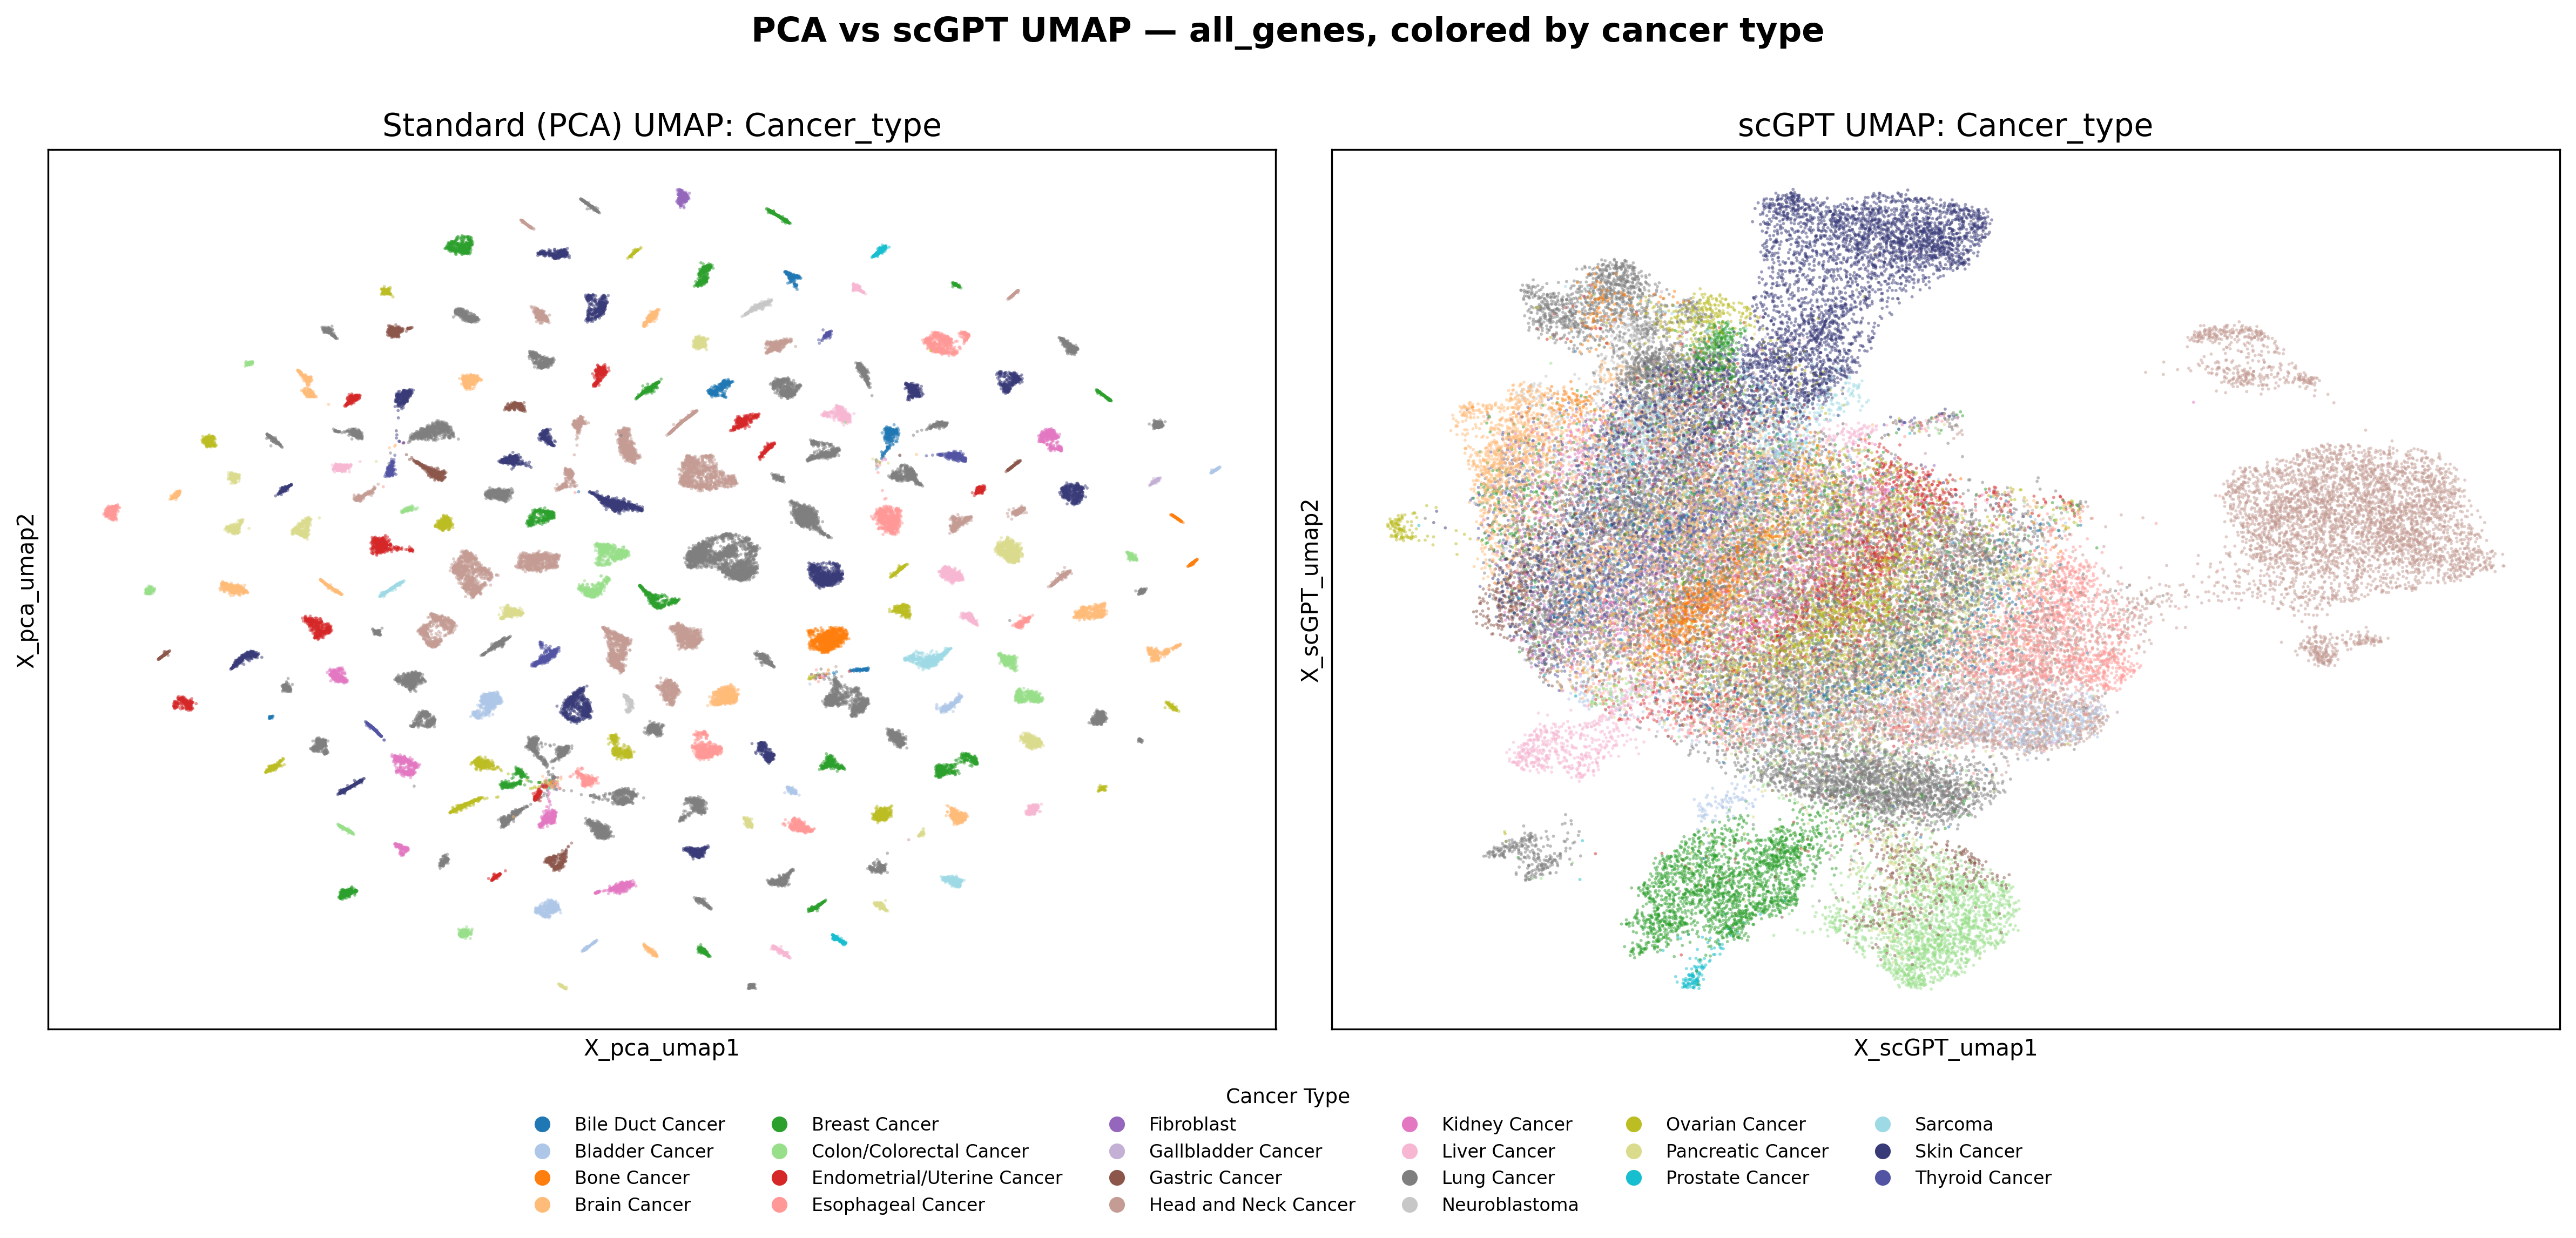
\includegraphics[width=0.9\textwidth]{fig_umap.png}
\caption{\textbf{scGPT removes the tissue-of-origin bias that dominates a PCA baseline.} Cells are embedded
by full-transcriptome PCA (left) and by scGPT (right), reduced to two dimensions by UMAP and colored by
cancer type. PCA separates the data into tissue-specific clusters, whereas scGPT projects the cells onto a
continuous, shared manifold. Produced by \code{notebooks/06\_verify\_variants.ipynb}.}
\label{fig:umap}
\end{figure}

\section{Methods}
+ scGPT erklären wie es funktioniert/trainiert
+ scGPT wieso? hypothese staten
\subsection{Data}

All experiments use the highest-confidence intersection of SCP542 \cite{scp542} and CTRPv2 \cite{ctrpv2,ctrp_rees}. This intersection comprises \NLines{} cell lines with
post-quality-control measurements (190 roster name matches, of which 10 are unscreened), \NDrugs{}
compounds and \NCells{} cells, with effectively complete viability coverage inside the overlap. Genes are
reduced to the \NHvg{} most highly variable; scGPT embeds the \NVocab{} of these that lie in its
vocabulary, while PCA is computed on all \NHvg{}. The gene-set size is not critical: an earlier sweep from
1{,}000 genes to the full transcriptome showed no advantage for any particular count
(\code{notebooks/07}), so the \NHvg-gene selection is used throughout.
\revision{\emph{Correction, 05.08.2026.} That sweep was computed on the legacy \code{mean\_pv} response
score rather than the \code{auc} target used throughout this report, so its numbers are superseded; it
now lives in \code{notebooks/data\_and\_harmonization/verify\_variants.ipynb}, \S9, and the reference to
\code{notebooks/07} above is stale. Its \emph{all-genes} arm is also not the full transcriptome as far as
scGPT is concerned: the model reads at most 1{,}200 genes per cell, drawn at random from that cell's
non-zero genes, so what the sweep compared was \NHvg{} \emph{selected} genes against a random subsample
of broadly similar size. The claim that gene-set size does not matter is therefore untested on the
current target.}

\begin{revisionblock}
\textbf{Expression preprocessing (revised 05.08.2026).} SCP542 is distributed as counts per million, so
library-size normalization has already been applied --- once, to the full gene matrix, which is where it
belongs. The pipeline therefore does not normalize a second time. Expression is log-transformed as
$\log(1+x)$; the \NHvg{} most variable genes are selected on that matrix using the dispersion-based
Seurat criterion; each gene is then standardized to zero mean and unit variance across cells, with
$z$-scores clipped at 10, before the principal components are taken
(\code{scripts/preprocessing/scp542\_conversion.py}, \code{scripts/preprocessing/add\_pca.py}).

Until this revision the PCA branch did two things differently. It applied a second library-size
normalization \emph{after} gene selection, dividing each cell by the total of its retained genes alone,
which rescales a cell by the share of its expression that happens to fall inside the selected set and
scales the same cell differently in each gene-set variant. And it applied no per-gene standardization,
so the leading components tracked absolute expression level rather than variation between cells. Both
are corrected in the code; \textbf{every PCA number in this report was produced before the correction}
and will change when the representation is recomputed.

scGPT receives the same CPM matrix with neither step applied. It replaces them with a per-cell binning
of expression into 51 quantile bins, computed from that cell's own non-zero values --- a rank transform,
and therefore invariant to any monotone per-cell rescaling. Counts, CPM and $\log(1+x)$ inputs give
identical bins, so the CPM input does not disadvantage the model \cite{scgpt}.
\end{revisionblock}

A property of the data governs every error estimate in this report. The label is defined per cell line and
drug, not per cell, so all cells of a line share the same broadcast bulk value and act as
pseudo-replicates. The effective sample size is therefore the number of cell lines, approximately
\NIndep{} after the held-out splits are removed, not the \NCells{} cells. Treating cells as independent
would understate the uncertainty by roughly the square root of the number of cells per line.

\subsection{Representation and model}

The comparison between representations is controlled so that only the content of the embedding differs.
Both the PCA baseline (\code{X\_pca}) and the scGPT embedding (\code{X\_scGPT}) are 512-dimensional and are
fed into the same multi-head perceptron, with hidden dimensions 128 and 64, layer normalization, GELU
activations and dropout. The network has one output head per drug and is trained with a masked
mean-squared-error loss that is evaluated only on observed cell-drug pairs. The model and training code are
defined in \code{scripts/model/OncoMLP.py} and \code{scripts/training/train\_multitask.py}.

\begin{revisionblock}
\textbf{Splits, and where each representation is fitted (added 05.08.2026).} Train, validation and test
are a 70/15/15 partition of cell lines, so every cell of a line falls on the same side and no line is
split across parts. The assignment is now \emph{frozen to a versioned file}
(\code{splits/split\_ctrp.csv}) instead of being redrawn from the data on each run. It has to be:
eligibility depends on which compounds survive the label filters, so a change to the drug panel would
otherwise move lines between train, validation and test unannounced, and results from either side of
that change would look comparable while being scored on different held-out lines. Redrawing requires an
explicit flag, and a line that the frozen file does not cover is an error rather than a fresh draw.

The principal components used as model input are fitted on the training lines of that split alone ---
per-gene standardization and the rotation both --- and then applied to the held-out lines
(\code{X\_pca\_train\_ctrp}). A separate all-cells decomposition (\code{X\_pca}) is kept for description
only, such as the latent-space figures, where holding cells out would be wrong. The cross-validation
results are the exception: its folds are drawn at training time rather than stored, so no precomputed
train-only projection exists for them and they still use the all-cells decomposition. scGPT needs no
such distinction --- its weights are pretrained and frozen, and its per-cell binning uses only the cell
being embedded, so nothing about it is fitted on this data.
\end{revisionblock}

\subsection{Response target and per-drug standardization}
\label{sec:target}

The choice of training target requires care. CTRPv2 provides a dose-averaged percent-viability score,
denoted \code{mean\_pv}, and an integrated area under the fitted dose-response curve, \code{auc}. The
initial experiments used \code{mean\_pv}; the final target is the curve-fit AUC standardized per drug
across cell lines, \code{auc\_z}, defined for cell line $i$ and drug $j$ as
$\mathrm{auc\_z}_{ij} = (\mathrm{auc}_{ij} - \mu_j)/\sigma_j$, where $\mu_j$ and $\sigma_j$ are the mean and
standard deviation of that drug's AUC over the cell lines.

Two considerations motivate the standardization. First, the per-drug response variance is highly
heterogeneous across the \NDrugs{} compounds, with the per-drug standard deviation ranging from 0.034 to
0.302, a factor of roughly 80 in squared error. In a shared multi-task objective with one masked
squared-error term per drug, the contribution of a drug scales with its variance, so a small number of
high-variance compounds dominate the shared representation irrespective of whether that variance carries
any learnable signal; the three drugs with the largest spread (\code{ifosfamide}, \code{fqi-2} and
\code{bafilomycin a1}) in fact fail to separate the cell lines at all. Standardizing each drug to unit
variance is algebraically equivalent to weighting each head by $1/\sigma_j^2$, which removes this
imbalance and is the regression analogue of loss reweighting under class imbalance \cite{kendall}. Second,
per-drug standardization changes the question from absolute potency, which is a property of the drug, to
the relative sensitivity of a cell line for a given drug, which is the quantity of interest for
personalized prediction. Because the Spearman correlation within a drug is invariant to an affine per-drug
transform, the standardization does not alter any single-drug evaluation metric; its only effect is on the
multi-task coupling. The target is implemented in \code{scripts/preprocessing/ctrp\_to\_h5ad.py}.

\subsection{Evaluation}

Cell lines are evaluated out of fold. A 5-fold group $k$-fold split, grouped by cell line, is applied to
the 153 training and validation lines, so that no cell of a test line is seen during training. Each line
is predicted exactly once, the per-cell predictions of a line are averaged to the line level, and the
Spearman correlation between predicted and true values across the roughly \NIndep{} lines is computed per
drug and averaged over drugs. This protocol replaces an earlier fixed 27-line validation split, on which
the standard error of a correlation is approximately 0.2 and effects below 0.4 are not measurable. The
Pearson correlation tracks the Spearman value within 0.02 throughout.

For external comparison, the model is additionally evaluated with the DrEval package \cite{dreval}
(version 1.5.1), using its leave-cell-line-out splits, its baselines and its evaluation routine without
reimplementation. As recommended by the framework, metrics are reported after the mean drug and cell-line
effects have been removed from both the true and predicted responses, and they are pooled over all
cell-line-drug pairs rather than averaged per drug, so they are not directly comparable to the per-drug
correlations above.

\section{Results}
\label{sec:results}

\subsection{Per-drug standardization is what makes the multi-task objective learnable}

Table~\ref{tab:target} compares the three targets across representations and head counts, with all other
settings fixed. On the subset of \NLearn{} learnable drugs the three targets are statistically
indistinguishable, which shows that the curve fit itself buys no accuracy over the dose average. The
difference appears only at the full \NDrugs-head scale: both unstandardized targets collapse to
approximately zero, with scGPT turning negative, whereas the standardized target retains
$\rho=\rhoFullScgpt{}$ (scGPT). Per-drug standardization is therefore a prerequisite for a learnable
large multi-task objective rather than a change to the information content of the label.

\begin{table}[t]
\centering
\caption{Out-of-fold Spearman correlation, averaged over the \NLearn{} learnable drugs, seed 42. The three
targets tie at K\,$=$\,\NLearn{}, but only the standardized \code{auc\_z} survives at K\,$=$\,\NDrugs{}.
Values are means of the per-drug rows in \code{outputs/target/target\_comparison.csv}
(\code{notebooks/11}).}
\label{tab:target}
\begin{tabular}{llccc}
\toprule
Heads & Representation & \code{mean\_pv} & \code{auc} & \code{auc\_z} \\
\midrule
\NLearn{} & PCA   & 0.370 & 0.360 & \rhoTenPca{} \\
\NLearn{} & scGPT & 0.396 & 0.405 & \rhoTenScgpt{} \\
\NDrugs{} & PCA   & $+0.073$ & $-0.012$ & \rhoFullPca{} \\
\NDrugs{} & scGPT & $-0.078$ & $-0.069$ & \rhoFullScgpt{} \\
\bottomrule
\end{tabular}
\end{table}

A set of single-parameter interventions on the unstandardized \NDrugs-head configuration locates the cause
(Figure~\ref{fig:rescue}). Starting from the broken baseline ($\rho=-0.08$), heavier regularization, a
smaller model, a different batch size and sample reweighting all leave the result unchanged or make it
worse. Two changes help. Removing the regularization recovers most of the gap (to $\rho=+0.21$), which
shows that the dropout had been interacting with the mis-scaled loss by starving the learnable heads of
shared capacity. Standardizing the target recovers the signal fully (to $\rho=+0.33$) without weakening the
regularization, which is why, once the target is corrected, regularization is flat and no longer a useful
lever.

\begin{figure}[t]
\centering
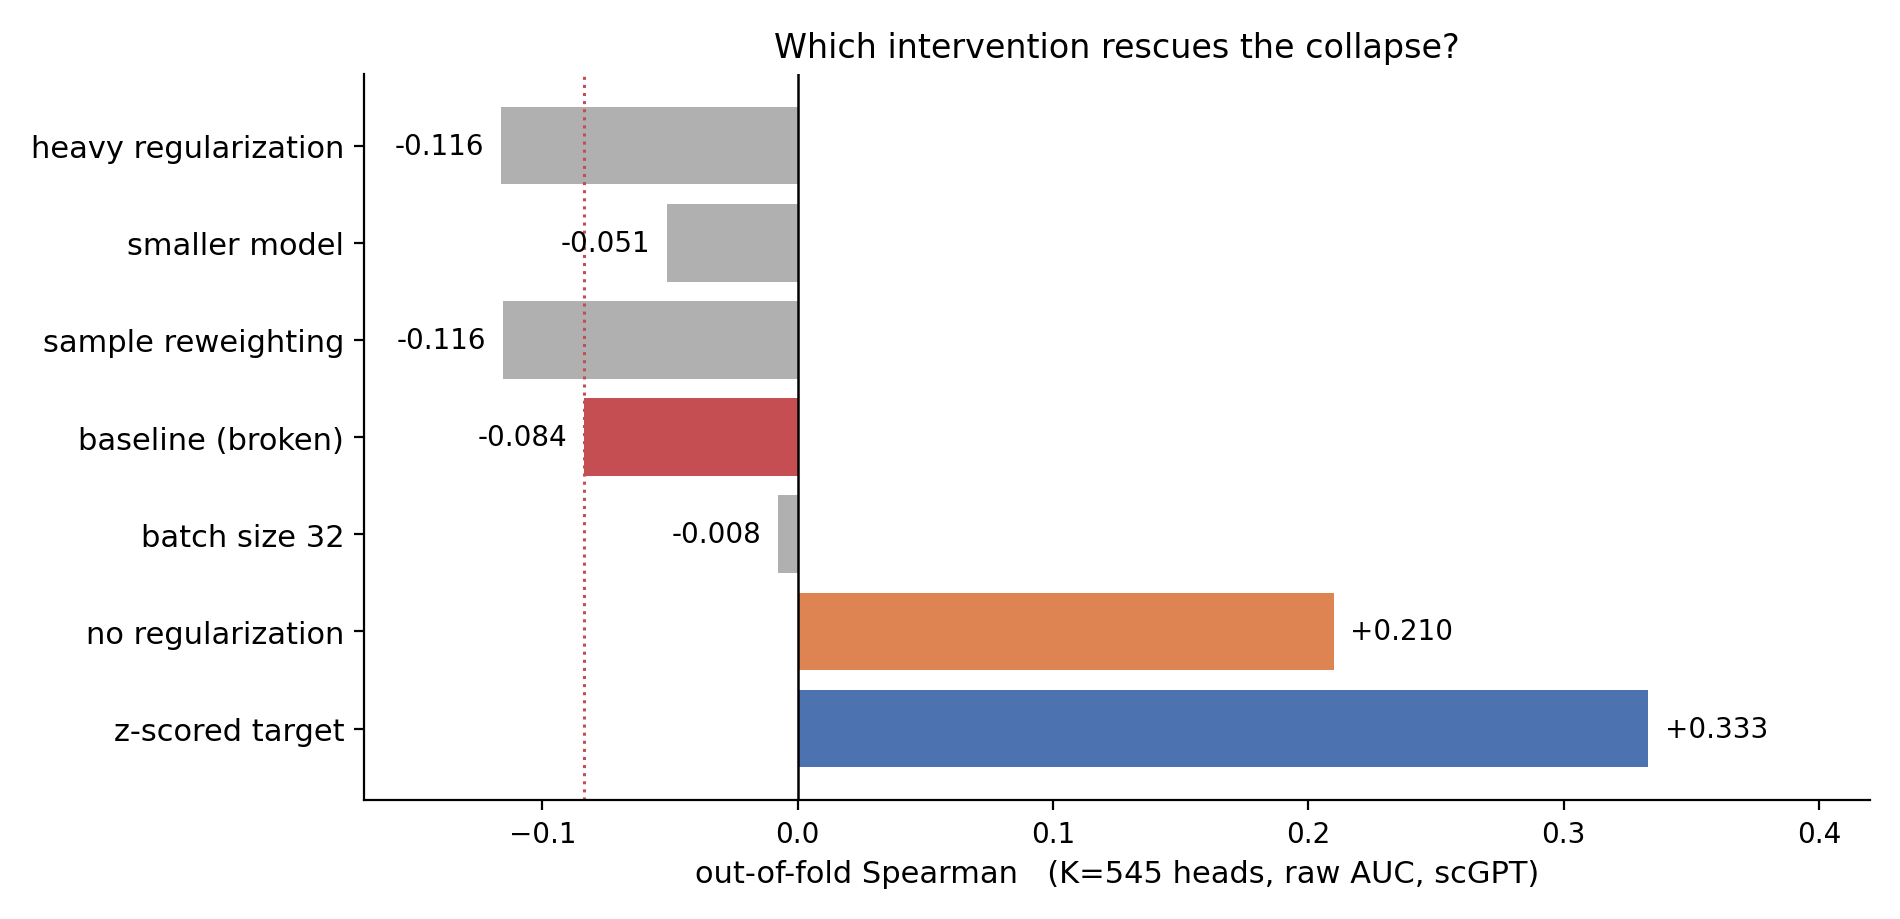
\includegraphics[width=0.78\textwidth]{fig_rescue.png}
\caption{\textbf{On the broken \NDrugs-head configuration, only removing regularization or standardizing
the target recovers the signal.} Each bar applies a single change to the same unstandardized setting (raw
\code{auc}, scGPT). Heavier regularization, a smaller model, a different batch size and reweighting (grey)
do not help; removing regularization (orange) recovers most of the gap; per-drug standardization (blue)
recovers it fully and addresses the cause. Source:
\code{outputs/ablations/rescue\_k545.png} (\code{notebooks/10}).}
\label{fig:rescue}
\end{figure}

\subsection{The corrected model ranks unseen cell lines at full head count}

With the standardized target the model ranks unseen cell lines well above chance. On the learnable subset
it reaches $\rho=\rhoTenScgpt{}$ (scGPT) and $\rho=\rhoTenPca{}$ (PCA), and it holds at
$\rho=\rhoFullScgpt{}$ and $\rho=\rhoFullPca{}$ even when all \NDrugs{} heads are trained jointly, which
shows that the large multi-task objective is trainable once the target is standardized.

\subsection{Model capacity is exhausted; the ceiling is the number of independent cell lines}

On the corrected setting, model-side tuning yields nothing further: regularization, capacity (from
\ParamsHi{} down to \ParamsLo{} parameters) and batch size all leave the correlation flat. The decisive
control is a ridge regression fitted to the \NIndep{} cell-line mean embeddings, with no single cells and
no network, which reaches $\rho=\ridgePca{}$ (PCA) and essentially ties the PCA multi-layer perceptron
($\rho=\mlpPcaR{}$). The deep single-cell apparatus adds a measurable margin only through scGPT
($\rho=\mlpScgptR{}$), and even there the scGPT signal is nonlinear, since a linear head on scGPT drops to
$\rho=\linScgptR{}$. The scGPT representation does, however, generalize better than PCA in the way the
guiding hypothesis predicts: sharing an identical trunk, its training-to-validation gap on the corrected
target is \gapScgpt{}, against \gapPca{} for PCA, so the foundation-model embedding overfits far less. The
limiting factor is thus the small number of independent cell lines and the noise of the broadcast labels,
not the representation or the architecture.

\subsection{Against the field, the model clears the naive baseline but not the best-in-class model}

Under the DrEval leave-cell-line-out protocol and its normalized metric (Table~\ref{tab:dreval},
Figure~\ref{fig:dreval}), our model exceeds the NaiveMeanEffects baseline that half of the published field
fails to beat, reaching a normalized Spearman correlation of \drScgptSp{} for scGPT against 0.000 for the
baseline, and it slightly exceeds DrEval's own SingleDrug reference models on identical features
($\rho=\drRfSp{}$ for their random forest). It remains below the best model the DrEval study reports, whose
normalized coefficient of determination reaches about \drPaperRsq{} against our \drScgptRsq{}. The
scGPT-over-PCA advantage seen in the internal evaluation shrinks to near noise once the mean effects are
removed (normalized Spearman \drScgptSp{} versus \drPcaSp{}). Consistent with the ridge control above, this
reproduces the study's central finding that most of the apparent performance in this field is the
cell-line and drug mean effect rather than differential response.

\begin{table}[t]
\centering
\caption{DrEval leave-cell-line-out benchmark, normalized metrics, mean over five folds. The model clears
the NaiveMeanEffects baseline and edges DrEval's reference models on identical features. Data source:
\code{outputs/dreval/dreval\_lco\_results.csv} (\code{notebooks/12}).}
\label{tab:dreval}
\begin{tabular}{lcc}
\toprule
Model & norm.\ Spearman & norm.\ $R^2$ \\
\midrule
NaiveMeanEffects (baseline) & 0.000 & 0.000 \\
SingleDrugRandomForest (scGPT) & \drRfSp{} & 0.098 \\
OncoMLP (X\_pca) & \drPcaSp{} & \drPcaRsq{} \\
OncoMLP (X\_scGPT) & \drScgptSp{} & \drScgptRsq{} \\
\bottomrule
\end{tabular}
\end{table}

\begin{figure}[t]
\centering
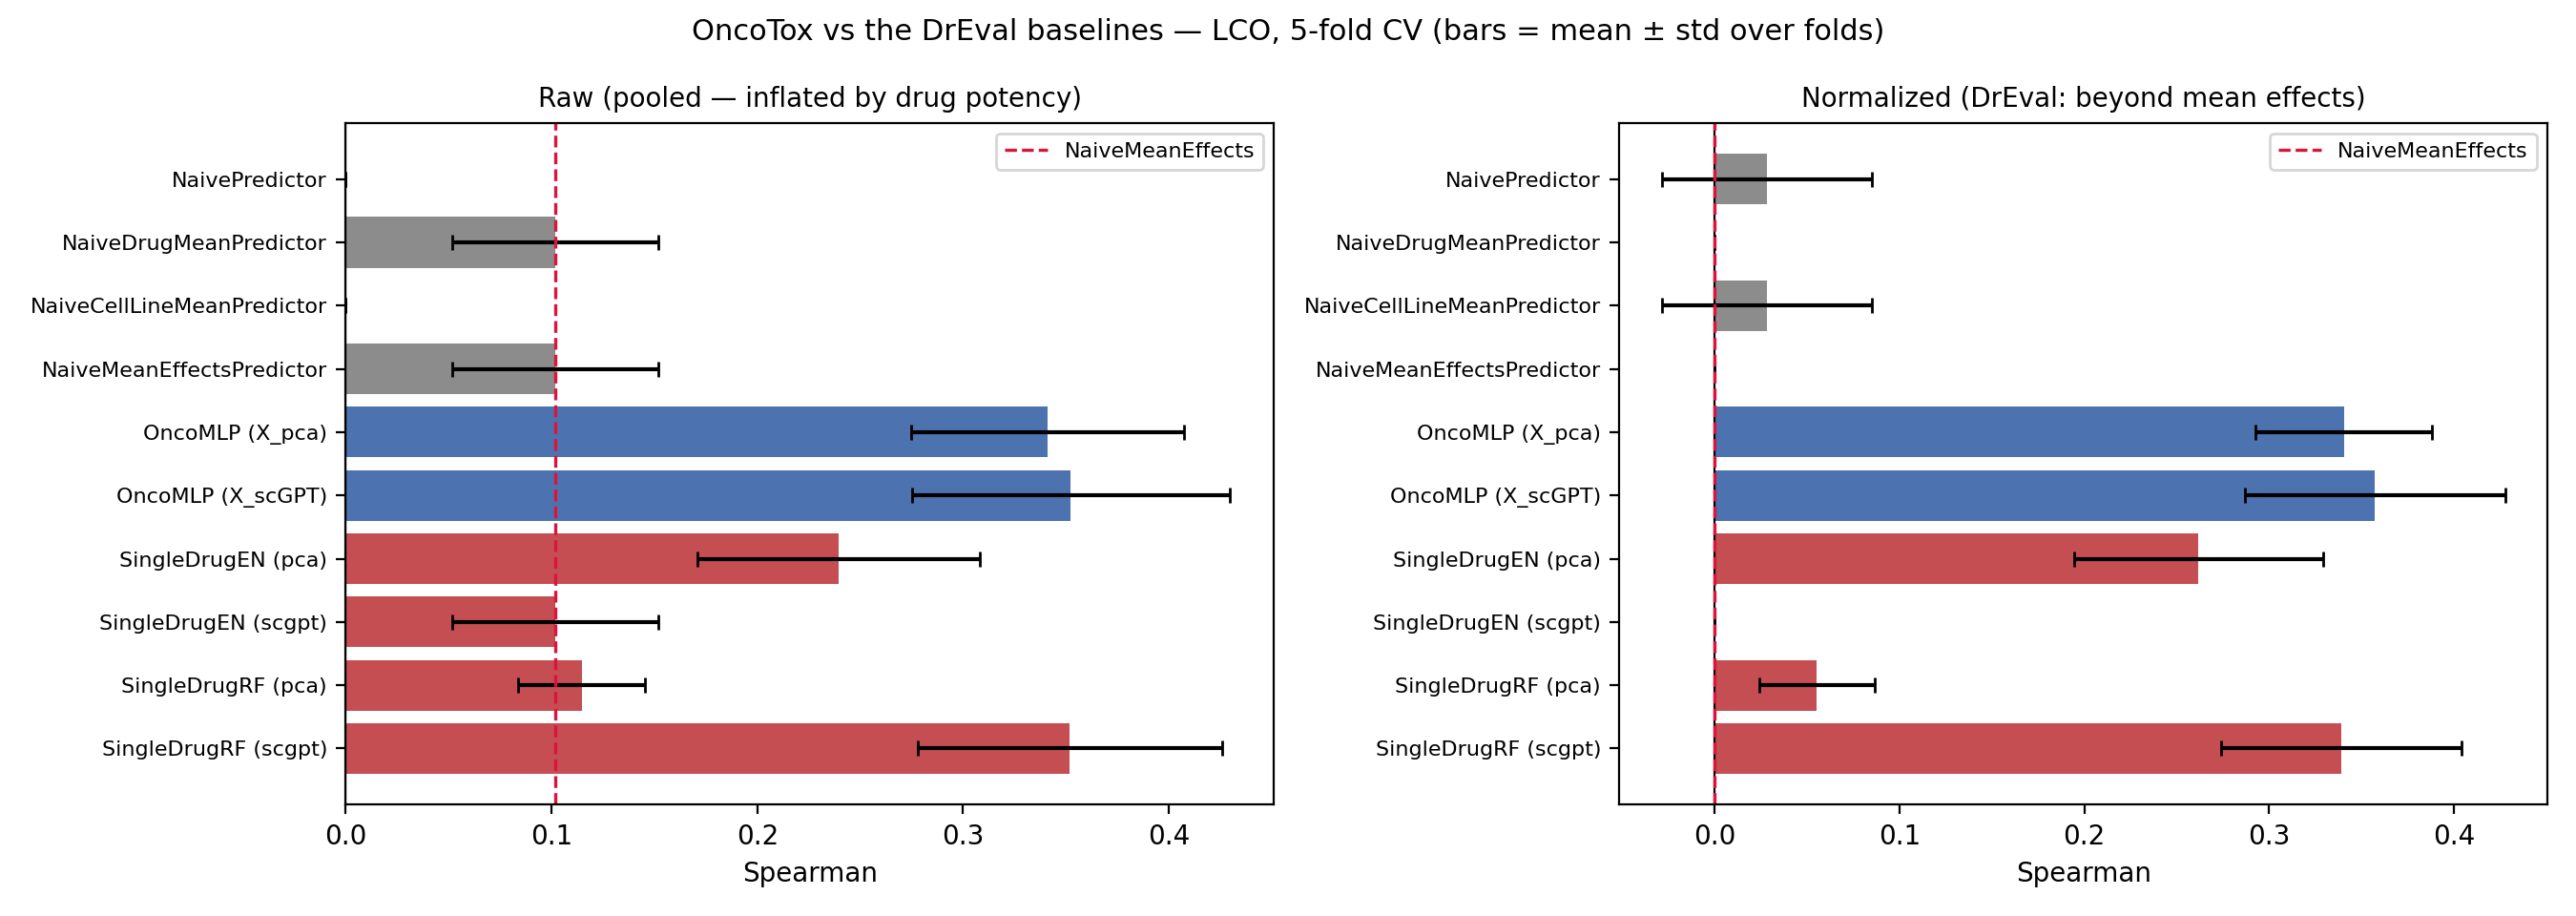
\includegraphics[width=0.9\textwidth]{fig_dreval.png}
\caption{\textbf{The naive predictors' raw performance is bias that the normalization removes.} DrEval
leave-cell-line-out results, raw pooled correlation (left) and normalized (right). The naive predictors sit
above zero on the left and collapse to zero on the right, which shows that their raw performance was the
mean effect; the model remains above the baseline after normalization. Source:
\code{outputs/dreval/dreval\_lco.png} (\code{notebooks/12}).}
\label{fig:dreval}
\end{figure}

\section{Discussion}

The results reframe an earlier, apparently negative finding. A first pass of this work had reported that
neither representation could rank cell lines, with out-of-fold correlations near zero over the full drug
panel. That outcome was substantially an artifact of the training target rather than a statement about the
data or the representation. The initial score, a dose-averaged viability, left the per-drug variances
untouched, so in the shared multi-task loss a handful of high-variance and largely uninformative
compounds dominated the representation. Standardizing the target per drug removes this imbalance, and with
it the model ranks unseen cell lines at correlations of \rhoFullScgpt{} across the panel and up to
\rhoTenScgpt{} on a learnable subset. The standardization is best understood as a necessary preprocessing
choice for a heterogeneous multi-task objective, not as a scientific result in itself; a head-to-head
comparison of the candidate scores is informative mainly because it shows that the curve fit alone changes
nothing and the standardization changes everything. The dominance of the target change is direct: on the
unstandardized targets the same model collapses at full head count (Table~\ref{tab:target}), and no other
single intervention on the broken configuration approaches it (Figure~\ref{fig:rescue}).

The corrected picture is modest but genuine, and it is best read against the standards the DrEval study
sets for the field. The model clears the NaiveMeanEffects baseline that about half of published models
fail to beat, and it edges DrEval's own reference models on identical features, but it remains below the best
model that study reports and shows only a faint representation advantage once the mean effects are
normalized away. The most informative internal result points the same way: a ridge regression on
cell-line mean embeddings matches the deep model, so the information the current pipeline exploits is
largely captured by a per-line average. This is the cell-line-effect bias that DrEval was designed to
expose, reproduced here independently. The single-cell resolution and the scGPT embedding together add a
small margin over that average, and scGPT needs a nonlinear head to realize it, which is the first
concrete evidence that the embedding carries structure a linear model cannot reach. This lower reliance on
memorization is the effect the guiding hypothesis anticipated, and it persists on the corrected target,
where the scGPT model's training-to-validation gap (\gapScgpt{}) is far smaller than that of PCA
(\gapPca{}) under an identical trunk.

Taken together, the evidence indicates that the limiting factor at this stage is the label side rather
than the model side. The task is defined on roughly \NIndep{} independent cell lines, each carrying one
bulk value broadcast onto hundreds of cells, and model-side tuning is exhausted across regularization,
capacity and batch size. Improving performance therefore requires acting on the labels and the data, not
on the architecture.

\section{Limitations and Future Work}

Several limitations bound the strength of the present claims, and each points to a concrete next step.

The most serious is that the learnable-drug subset was selected using all \NLines{} cell lines, including
the validation and test lines, so any number reported on that subset is a best-case diagnostic rather than
a generalization estimate; the selection should instead be performed inside each cross-validation fold,
using only the training lines. The subset is moreover chosen from label statistics alone and was not
validated in this report against the per-drug performance the model actually achieves, so it should be
read as a diagnostic device rather than a claim that only ten drugs are learnable.

The scGPT advantage over PCA is small: a Spearman gap of $+0.036$ at K\,$=$\,\NLearn{} and $+0.012$ at
K\,$=$\,\NDrugs{}, of the same order as the seed-to-seed variation. Across three seeds the gap averages
$+0.04$ and is not sign-consistent, ranging from $-0.00$ to $+0.09$, and it does not survive DrEval's
normalized metric, so it should not be presented as an established margin until it has been reproduced over
more seeds and a wider drug set. The external benchmark is itself preliminary, covering only the
leave-cell-line-out split on the learnable subset rather than the leave-tissue-out and leave-drug-out
settings or the full panel.

The clearest opportunities for improvement follow from the diagnosis that the task is label-limited. First,
the training target can be aligned with the evaluation by regressing on the doubly normalized residual, in
which both the drug and the cell-line mean effects are removed, with the means estimated only on the
training lines of each fold; this matches the quantity DrEval rewards, and an initial check
(\code{outputs/dreval/dreval\_normalized.csv}) indicates that about a fifth of the current signal is the
cell-line effect alone. Second, the single-cell resolution has
yet to justify itself, since averaging a line's cells loses nothing measurable; a pooling model that
predicts the line label from a bag of cells, for example through attention, is the natural test and must
beat the ridge control to be worthwhile. Third, and most directly, the ceiling can be raised by adding
independent cell lines, as CTRPv2 alone screens roughly 1{,}100 against the \NLines{} in the current
overlap. Beyond these, a diagnostic error analysis of where the model fails is low-risk and immediately
useful, whereas gene-level interpretation to surface transcriptomic drivers of resistance is worthwhile
only once per-drug performance is substantially higher and stable, so that the interpretation does not
merely describe noise. The longer horizon remains a cross-database, multi-task model spanning
efficacy and toxicity, fine-tunable on clinical outcomes.

\begin{thebibliography}{9}

\bibitem{ctrp}
Seashore-Ludlow, B.\ et al.
Harnessing connectivity in a large-scale small-molecule sensitivity dataset.
\textit{Cancer Discovery} \textbf{5}, 1210--1223 (2015);
and Rees, M.~G.\ et al.
Correlating chemical sensitivity and basal gene expression reveals mechanism of action.
\textit{Nature Chemical Biology} \textbf{12}, 109--116 (2016).

\bibitem{prism}
DepMap, Broad; Kocak, M.
Repurposing Public 24Q2. figshare dataset (2024).
\url{https://doi.org/10.6084/m9.figshare.25917643.v1}

\bibitem{gdsc}
Genomics of Drug Sensitivity in Cancer (GDSC), Wellcome Sanger Institute.
\url{https://cellmodelpassports.sanger.ac.uk/downloads}

\bibitem{scp542}
Kinker, G.~S.\ et al.
Pan-cancer single-cell RNA-seq identifies recurring programs of cellular heterogeneity.
\textit{Nature Genetics} \textbf{52}, 1208--1218 (2020).
\url{https://doi.org/10.1038/s41588-020-00726-6}

\bibitem{perception}
Sinha, S.\ et al.
PERCEPTION predicts patient response and resistance to treatment using single-cell transcriptomics of
their tumors.
\textit{Nature Cancer} \textbf{5}, 938--952 (2024).
\url{https://doi.org/10.1038/s43018-024-00756-7}

\bibitem{scgpt}
Cui, H.\ et al.
scGPT: toward building a foundation model for single-cell multi-omics using generative AI.
\textit{Nature Methods} \textbf{21}, 1470--1480 (2024).
\url{https://doi.org/10.1038/s41592-024-02201-0}

\bibitem{dreval}
Bernett, J., Iversen, P., Picciani, M., Wilhelm, M., Baum, K.\ \& List, M.
Critical evaluation of drug response prediction models with DrEval.
\textit{Nature Communications} (2026). Software: \code{drevalpy} v1.5.1.

\bibitem{kendall}
Kendall, A., Gal, Y.\ \& Cipolla, R.
Multi-task learning using uncertainty to weigh losses for scene geometry and semantics.
\textit{IEEE Conference on Computer Vision and Pattern Recognition (CVPR)} (2018).

\end{thebibliography}


\end{document}
